\chapter{System Architecture}
\noindent\rule{\linewidth}{2pt}
This chapter describes the overall system architecture of CropLens AI, explaining how the frontend, backend, machine learning pipeline, AI explanation engine, and external services interact to deliver a complete crop health assessment.

\section{Architecture Overview}

CropLens AI follows a three-layer client--server architecture:
\begin{enumerate}
    \item \textbf{Presentation Layer:} React 19 + Vite single-page application (SPA) running on \texttt{localhost:5173} during development.
    \item \textbf{Application Layer:} FastAPI Python backend running on \texttt{localhost:8000}. Loads all ML models at startup and exposes REST and SSE endpoints.
    \item \textbf{Data and Inference Layer:} PyTorch-based neural network models, scikit-learn Random Forest, deterministic Risk Fusion Engine, Gemini REST API, and Open-Meteo weather API.
\end{enumerate}

\section{Frontend Architecture (React + Vite)}

The frontend is a hash-routed SPA with six distinct views:
\begin{itemize}
    \item \textbf{LandingView.jsx:} Hero section with a Three.js 3D ambient canvas, key system statistics, and navigation.
    \item \textbf{ScanView.jsx:} Upload form accepting a leaf image and farm parameters (N, P, K, fertilizer, temperature, location, soil type, pH, farm area, rainfall).
    \item \textbf{ProcessingView.jsx:} Real-time animated eight-stage pipeline timeline driven by SSE events from the backend.
    \item \textbf{CropHealthReport.jsx + AIAssistant.jsx:} Comprehensive report with diagnostic summary, KPI cards, weather context, Gemini explanation, and a vertical infographic timeline.
    \item \textbf{ArchitectureView.jsx:} Interactive pipeline diagram with clickable component detail panels.
    \item \textbf{ResearchView.jsx:} Research evidence page with dataset cards, benchmark metrics table, and verified academic paper references.
\end{itemize}

\section{Backend Architecture (FastAPI)}

The FastAPI backend implements the following key endpoints:
\begin{itemize}
    \item \textbf{POST /predict/crop-health/stream:} Server-Sent Events streaming endpoint. Runs the full ML pipeline and emits JSON events for each stage.
    \item \textbf{POST /predict/crop-health:} Standard REST fallback endpoint returning the complete analysis result as a single JSON response.
    \item \textbf{POST /explain/crop-health:} Gemini explanation endpoint. Accepts structured prediction data, retrieves the knowledge base entry, and returns a Gemini-generated or deterministic disease-specific explanation.
    \item \textbf{GET /health:} Health check endpoint.
\end{itemize}

All four ML models are loaded into memory at application startup to avoid per-request loading latency.

\section{System Architecture Diagram}

Figure~\ref{fig:sys_arch} illustrates the complete system architecture diagram of CropLens AI, showing the end-to-end integration from leaf image acquisition to final multi-signal decision report.

\begin{figure}[H]
\centering
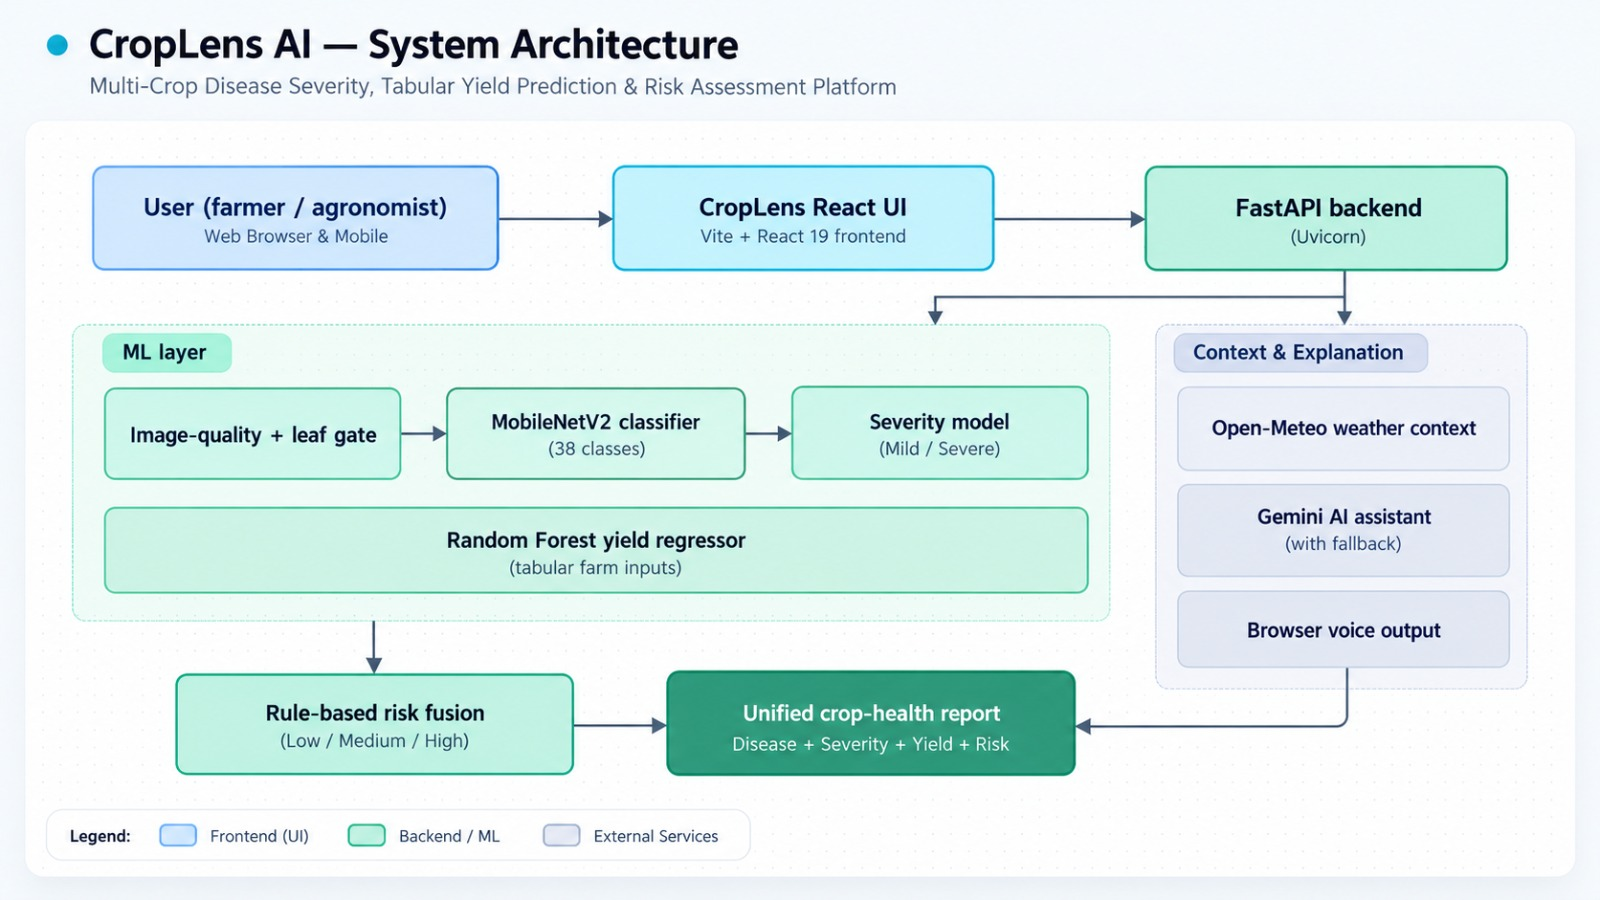
\includegraphics[width=0.95\textwidth]{Figures/system_architecture_ppt.png}
\caption{CropLens AI Complete System Architecture Diagram}
\label{fig:sys_arch}
\end{figure}

\FloatBarrier

\section{End-to-End System Workflow Architecture}

Figure~\ref{fig:workflow_arch} illustrates the workflow and data flow architecture of CropLens AI, following the modular hub-and-spoke layout connecting user interactions, neural classifiers, regressors, and explanation services.

\begin{figure}[H]
\centering
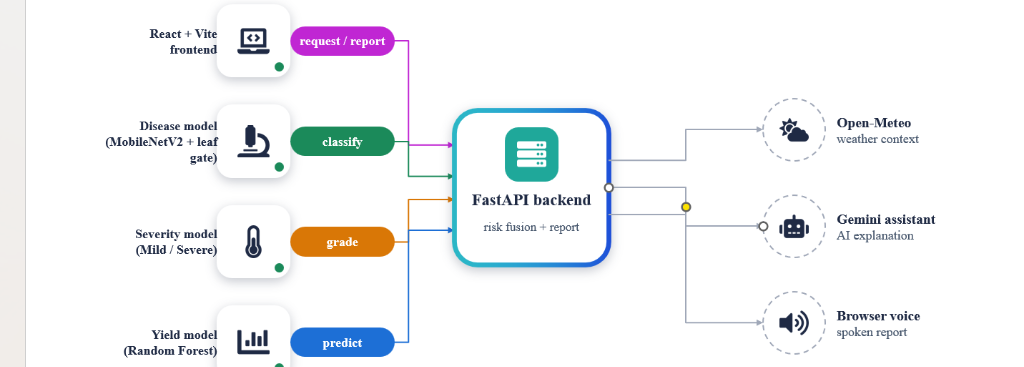
\includegraphics[width=0.92\textwidth]{Figures/workflow_architecture.png}
\caption{CropLens AI End-to-End Workflow Architecture}
\label{fig:workflow_arch}
\end{figure}

\FloatBarrier

As shown in Figure~\ref{fig:workflow_arch}, the workflow comprises:
\begin{enumerate}
    \item \textbf{Client Input (React + Vite):} The user submits a leaf photograph and agronomic parameters through the web frontend.
    \item \textbf{Inference Pipeline Components:}
    \begin{itemize}
        \item \textbf{Disease Model (MobileNetV2 + Leaf Gate):} Validates that the uploaded image contains plant foliage, then classifies the crop and disease across 38 classes.
        \item \textbf{Severity Model (Mild / Severe):} Applies disease-conditioned classification on supported crop-disease pairs.
        \item \textbf{Yield Model (Random Forest):} Predicts expected yield in tonnes per hectare from tabular soil and climate parameters.
    \end{itemize}
    \item \textbf{FastAPI Backend (Risk Fusion + Report):} Central coordination engine that validates incoming requests, runs the ML models sequentially, fuses disease severity and yield risk into a unified risk rating, and compiles the final report.
    \item \textbf{Context and Explanation Services:}
    \begin{itemize}
        \item \textbf{Open-Meteo:} Provides live regional weather context (temperature, humidity, precipitation).
        \item \textbf{Gemini Assistant:} Translates structured prediction outputs into plain-language agronomic explanations grounded in extension service knowledge.
        \item \textbf{Browser Voice:} Converts the diagnostic report into synthesized speech for accessible voice narration.
    \end{itemize}
\end{enumerate}

\section{Disease-Conditioned Severity Model Architecture}

The \texttt{DiseaseConditioned-}\allowbreak\texttt{MobileNetV2} architecture combines:
\begin{itemize}
    \item A MobileNetV2 backbone producing a 1,280-dimensional image feature vector via global average pooling.
    \item A learned \texttt{nn.Embedding} layer mapping disease pair ID (0--13) to a 32-dimensional disease vector.
    \item Concatenation of the 1,280-dim image feature and 32-dim disease embedding (1,312 total dimensions).
    \item A two-layer classifier head (Linear $\rightarrow$ ReLU $\rightarrow$ Dropout $\rightarrow$ Linear $\rightarrow$ 2 classes) producing Mild or Severe logits.
\end{itemize}

\section{AI Explanation Engine Architecture}

The Gemini explanation engine operates as follows:
\begin{enumerate}
    \item Frontend sends a POST request to \texttt{/explain/crop-health} with structured prediction data (crop, disease, confidence, severity, yield, risk).
    \item Backend resolves the knowledge base entry for the detected disease.
    \item A structured prompt is constructed combining prediction results and relevant knowledge base facts.
    \item Gemini (\texttt{gemini-3.5-flash-lite}) generates a structured JSON explanation covering eight sections: disease overview, favorable conditions, symptoms, transmission, prevention, management, severity interpretation, and professional advice triggers.
    \item The JSON is validated and returned to the frontend for display in the vertical infographic timeline.
    \item If Gemini is unavailable, a deterministic fallback builds an equivalent explanation from the knowledge base.
\end{enumerate}

\section{Streaming Architecture (Server-Sent Events)}

The FastAPI backend uses an asynchronous generator \texttt{run\_crop\_health\_pipeline()} that yields Server-Sent Events (SSE) formatted as \texttt{data: \{stage, status, result\}}. The browser reads this continuous stream using the Fetch API and \texttt{ReadableStream}, updating the React pipeline view in real time as each stage completes.

\section{Database and Model Storage Design}

CropLens AI does not require an external database server. All model weights and knowledge representations are stored as versioned files:
\begin{itemize}
    \item \texttt{ml-service/models/leaf\_gate\_mobilenetv2\_best.pth} --- Leaf Gate weights.
    \item \texttt{ml-service/models/disease\_mobilenetv2\_best.pth} --- Disease Classifier weights.
    \item \texttt{ml-service/models/severity\_conditioned\_mobilenetv2\_best.pth} --- Severity Model weights.
    \item \texttt{ml-service/models/yield\_model.pkl} --- Serialized Random Forest Regressor.
    \item \texttt{ml-service/knowledge\_base.py} --- Structured dictionary of 38 disease entries.
\end{itemize}

\section{Summary}

This chapter presented the layered system architecture, complete system architecture diagram from the project, end-to-end workflow diagram matching the reference design, and the file-based model storage mechanism. The decoupled frontend, streaming API, and deterministic fallback design ensure high reliability and responsive user experience.
